\section{Travelling Wave Analysis}

%%%%%%%%%%%%%%%%%%%%%%%%%%%%%%%%%%%%%%%%%%%%%%%%%%%%%%%%%%%
\subsection{Spatial Simplification}

To simplify the travelling wave analysis we reduce the spatial dimensions to that of a 1D problem.
This can be done if initial conditions that are homogenous with respect to $y$ are choosen.
The purpose of this spatial simplification is that this will speed up the computations considerable.
It will also make visualizations easier as certain figures would become too cluttered in 2D.
What is done here is more of a psuedo-reduction of dimensions.
By reducing the grids from an $n \times m$ grid to an $n \times 4$ grid we have changed the way the problem size scales with finer grids.
The problem is still 2D, just now one dimension has been reduced to only 4 grid points of accuracy instead of $m$ points.
This does not effect the final result since we only apply this change to problems with appropriate initial conditions.
These initial conditions are homogenous in the $y$ direction and thus we do not have any fluctuation between $y$ values for a given $x$ value.

One main benefit of changing the grid from $n \times m$ to $n \times 4$ is that the growth of the problem with respect to the resolution of the grid is reduced dramatically.
This changes the problem from a $O(n^2)$ problem to a $O(n)$.
Using the travelling wave 1D initial conditions one simulation is computed with a $513 \times 513$ grid, seen at Figure \ref{fig:show_dimension_3D}, and another with a $513 \times 4$ grid, seen at Figure \ref{fig:show_dimension_2D}.
% Use the below version, has reference
%!%Using the travelling wave 1D initial conditions, (\ref{equ:basic_init_trav_wave}), one simulation is computed with a $513 \times 513$ grid, seen at Figure \ref{fig:show_dimension_3D}, and another with a $513 \times 4$ grid, seen at Figure \ref{fig:show_dimension_2D}.

\begin{figure}[h!bt]
  \centering
  \begin{tabular}{c c}
    \includegraphics[scale=0.7]{show_dimension_3D.eps} &
    \includegraphics[scale=0.7]{show_dimension_3D_side.eps} \\
    (a) & (b) \\
  \end{tabular}
  \caption{Graph of (a) 3D view of $M(t,x,y)$ and $C(t,x,y)$, (b) Side profile view of $M(t,x,y)$ and $C(t,x,y)$ at $t=40$.} 
  \label{fig:show_dimension_3D}
\end{figure}
   
Before any changes to the grid can be made, it must be confirmed that fluctuations are sufficently small.
To this end, the standard deviation is used as a measure.
The standard deviation is calculated along the $y$-direction for each x value.
This gives a numerical quantity for the measure of dispersal each $y$ value has with another.
Here, we use the sample standard deviation for the sole reason that this single simulation does not represent its own population.
Initially, at $t =0$ the standard deviation is 0 everywhere (DATA NOT SHOWN).
At $t = 40$, Figure \ref{fig:show_dimension_stddev} show the standard of each y value.
After many timesteps have passed the amount of spread is always less then $10^{-14}$, which is an acceptable degree of consistency.
Note that the main inconsistency is at the wave front, around $x = 5.75$, which is mainly because of the sharp change in values.

\begin{figure}[h!bt]
  \centering
  \includegraphics{show_dimension_stddev.eps}
  \caption{The standard deviation at the same time as the above graphs}
  \label{fig:show_dimension_stddev}
\end{figure}


%!% I don't this this is anymore stronger then the std dev example.
  %    This can be shown quantitatily by comparing the maximum and minimum values of M and C with respect to the x-axis (Figure \ref{fig:maxMin}). 
  %  \begin{figure}[h!bt]
  %    \begin{center}
  %        \includegraphics[scale=0.8]{maxMin_MC.eps}
  %      \caption{Graph of difference between max and min of M and difference between max and min of C.}
  %      \label{fig:maxMin}
  %    \end{center}
  %  \end{figure}
  %
  %  %!% Reverse the order of this; show calculation before the table.
  %  The difference between the max and min remains constant with respect to time (Table \ref{tab:overTime}), this was calculated by,
  %  \begin{equation}
  %    \begin{aligned}
  %      \delta_M(t) &= \frac{1}{256}\sum_{i = 1}^n \left( \sup_{j \in (1,m)} M(x_i,y_j) - \inf_{k \in (1,m)} M(x_i,y_k) \right) \\
  %      \delta_C(t) &= \frac{1}{256}\sum_{i = 1}^n \left( \sup_{j \in (1,m)} C(x_i,y_j) - \inf_{k \in (1,m)} C(x_i,y_k) \right)   
  %    \end{aligned}
  %  \end{equation}
  %  
  %   \begin{table}
  %    \begin{center}
  %      \begin{tabular}{| c | c | c |} 
  %        \hline
  %        t & $\delta_M$ & $\delta_C$ \\
  %        \hline
  %        0.0 & 0.0 & 0.0037109375 \\
  %        0.5 &1.71577851563e-06 & 0.00371116503633\\
  %        1.0 &7.62408671875e-06 & 0.00371156747773\\
  %        1.5 &9.04633828125e-06 & 0.00371216829336\\
  %        2.0 &7.648728125e-06 & 0.00371311224609\\
  %        2.5 &2.58707890625e-06 & 0.00371457725742\\
  %        3.0 &0.00162623974609 & 0.00240237613672\\
  %        3.5 &5.35270417969e-05 & 7.24265101562e-05\\
  %        4.5 &1.07250539062e-05 & 2.12679726563e-05 \\
  %        5.0 &1.09254414063e-06 & 9.720734375e-06\\
  %        \hline
  %      \end{tabular}
  %      \caption{A table of values for $\delta_M(t)$ and $\delta_C(t)$}
  %      \label{tab:overTime}
  %    \end{center}
  %  \end{table}
   
When simulations are computed with a $n \times 4$ grid, they are still 2D problems.
With regards to visualizations, side profiles could be used on these solutions to present psuedo-1D visualization but this is not ideal.
To visualize the solutions in true 1D the we use $\bar{M}$ and $\bar{C}$ as averaged values of the solutions along the y-axis.
This is computed after the solution has been determined and is independent of the actual compuations for M and C.
So by taking the average of the points along the $y$-axis we can get a 2D plot as seen in Figure \ref{fig:show_dimension_2D}. 
 
\begin{figure}[h!bt]
  \begin{center}
    \includegraphics{show_dimension_2D.eps}
    \caption{Graph of M(2,y) and C(2,y), now reduced to a 2D plot.}
    \label{fig:show_dimension_2D}
  \end{center}
\end{figure}

This means that the system can be reduced to a $1D$ problem.
%!%This means that the system (\ref{equ:model_system} - \ref{equ:model_functions}) can be reduced to a $1D$ problem. 
With initial conditions that are homogenous with respect to y, we can greatly reduce the accuracy in the one axis.
Once the y-axis reduced, we can also ignore it for visualizations, only using the x-z axis and plotting the values of $\bar{M}$ and $\bar{C}$.


%%%%%%%%%%%%%%%%%%%%%%%%%%%%%%%%%%%%%%%%%%%%%%%%%%%%%%%
\subsection{Travelling Wave Solution}


%!% section 1.2.2 i think before you discuss travelling waves, you should define what they are. Just take it from my old paper
Classical travelling wave solutions are solutions that propagate with an \textit{a priori} unknown constant speed without any change in shape.
This means that the solutions can be defined as 
\begin{equation}
  M(t,\tilde{x}) = M(\tilde{x} - ct)
\end{equation}
Figure \ref{fig:trav_wave_solution} shows the time evolution of the single time snapsnot from Figure \ref{fig:show_dimension_2D}.
Given the above definition and by looking at the consistent appearence of the solution, it suggests that it is a travelling wave.
It is clear here that the shape of the solution is consistent enough to suggest the existence of a travelling wave solution.

\begin{figure}[h!tb]
\begin{center}
  \begin{tabular}{c c}
      \includegraphics[scale=0.55]{trav_wave_solution_t0.eps} &
      \includegraphics[scale=0.55]{trav_wave_solution_t20.eps} \\
      (a) & (b) \\
      \includegraphics[scale=0.55]{trav_wave_solution_t40.eps} & 
      \includegraphics[scale=0.55]{trav_wave_solution_t60.eps} \\
      (c) & (d) 
  \end{tabular}
  \caption{Solutions of $M(x,t)$ and $C(x,t)$ at (a) t = 0, (b) t = 20, (c) = 40, (d) = 60. 
    This was run on a $513 \times 4$ grid.}
  \label{fig:trav_wave_solution}
\end{center}
\end{figure}

The existance of a travelling wave solution for this simulation can be confirmed if the solution $M(x,t)$ can be shown as $M(x-ct)$, where $c$ is the \textit{a priori} unknown wavespeed.
Visually, multiple timesteps horizontally translated onto each other would show this.
If the horizontal translations are all multiples of the same number then we have shown that a constant speed exists.
If the shape of all the timesteps match then a constant shape then strong evidence that a constant shape exists would be shown.
We can numerically approximate the value for $c$ by looking at how fast the peak of the wave travels.
The location of the wave peak is the x coordinate that corresponds to the largest $M$ value.
Recall that we are dealing with a psuedo-1D problem, so there does not need to be any consideration for an $(x,y)$ coordinate.
For this case, we used the GNUPLOT software to fit a linear model, $f(x) = mx + b$, to the last half of the wave peaks path, seen in Figure \ref{fig:trav_waveSpeed}.
The last half of the values were used instead of the whole set of values because only for the former do we have a fully formed travelling wave.
The value of $m$ in $f(x)$ is the approximation for the wavespeed, $c$. 

\begin{figure}[h!tb]
\begin{center}
    \includegraphics[scale=0.85]{trav_wavespeed.eps}
    %!% At some point, try to get a line in the graphic that show the region that was used for the fitting.
    \caption{The $x$ location of the wave peak as a function of $t$.
      The red line is the wave peak location extracted from the simulation results.
      The green line is the function $f(x) = cx + b$ with c as the wavespeed, found by fitting the model to the second half of x values.
      The simulation results used here are from the solution shown in the previous Figure.
    }
    \label{fig:trav_waveSpeed} 
\end{center}
\end{figure}

With an approximation for $c$, the solutions of Figure \ref{fig:trav_wave_solution} can be represented as $M(x - c (t_0 - t_{n}))$, where $t_0 = 60$ is a reference point for the other timesteps.
The values of $t_{n}$ are the times for the other solutions.
By translating along the $x$-axis multipl solution profiles can be superimposed, as seen in Figure \ref{fig:trav_wave_translation}.
The shape of each timestep is very similar throughout, only differing slightly at the tail.

\begin{figure}[h!tb]
\begin{center}
    \includegraphics[scale=0.85]{trav_wave_translation.eps}
    %!% Fix this caption here. The variables don't mke sense anymore
    \caption{Solutions of $M$ that are represented as $M(x -ct)$ \textit{a priori}.
      The multiple timesteps are translated on top of another by horizontal movements of $c (t_0 - t_n)$ for each timestep.
      }
    \label{fig:trav_wave_translation}
\end{center}
\end{figure}

Based on the above evidence, we can say that a travelling wave solution has been shown to exist for a single initial condition and particular set of parameters.
This leads to two logical extensions, looking at the stability of the travelling wave solution based on initial condition and investigating the effect the parameters have on the travelling wave solution.

%%%%%%%%%%%%%%%%%%%%%%%%%%%%%%%%%%%%%%%%%%%%%%%%%%%%%%%%%%%
\subsection{Travelling Wave Stability}

%!% section 1.2.3:  it seems that you are here interested in whether you obtain a 1D travelling wave, i.e. you measure whether your solution deviates from a 1D solution. I am not certain that this is the relevant question. I think the question is whether in a full 2D case you get a travelling wave (which does not need to be a 1D wave but can be a fully 2D solution). Your figure \ref{trav_wavefront} seems to suggest this. We can talk about this in the exam or next week.

Based on the previous example, there seems to exist a travelling wave solution. %!% for the intial condition given in (\ref{equ:basic_init_trav_wave}).
The next step is looking at how different initial conditions could still result in a travelling wave solution.
For this we specifically look at the stability of the solution, does it attact nearby solution into becoming a travelling wave solution or is it only for specific cases that one results.
This will help confirm that the existence of the travelling wave solution is not depended on the single choice of initial condition.

To test this we take an initial condition that is not inherently one dimensional and see if it approches to the one dimension property.
The choice of IC is to have multiple random spherical innoculation points along the $y=0$ side of the region.
Specifically, we use $(x_r, y_r)$ to represent the center of each random innoculation point.
Here $x_r \in \mathcal{R}$ and $y_r \in [0, 0.1]$.

The equation used for each random spherical innoculation point is,
\begin{equation}
  M = \frac{-h}{d^2} \left( (x - x_r)^2 + (y - y_r)^2 \right) + h, \quad M \ge  0.
\end{equation}
Random innoculation points add to each other if they overlap.
After all the innoculation points have been generated, every value is divide by the total amount of biomass.
This lets the initial condition become a representation for the distribution of random innoculation points in terms of the total amount generated.
A time evolution of the simulation with the above initial condition can been seen in Figure \ref{fig:trav_stability}.
Here it can be observed that the solution $M$ appears to slowly converge to a 1D problem.
This cannot be fully seen since the wave propagation reachs the end of the region before it can become fully one dimensional.

\begin{figure}[h!tb]
  \centering
  \begin{tabular}{c c}
      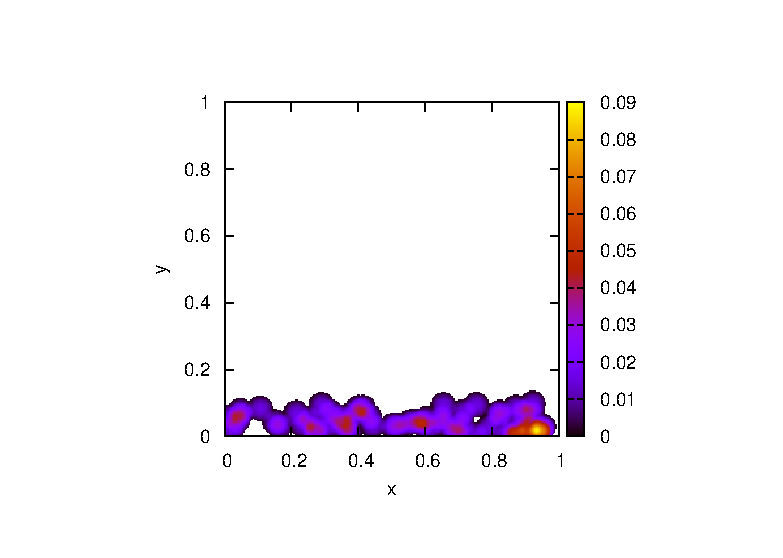
\includegraphics[scale=0.55]{trav_stability_t0.eps} &
      \includegraphics[scale=0.55]{trav_stability_t10.eps} \\
      (a) & (b) \\
      \includegraphics[scale=0.55]{trav_stability_t20.eps} &
      \includegraphics[scale=0.55]{trav_stability_t30.eps} \\
      (c) & (d) 
  \end{tabular}
  \caption{Plots of the simulation with random spherical innoculation points centered in the region $(x,y) \in [0,0] \times [1,0.1]$.
    The solutions are shown at (a) $t = 0$, (b) $t = 10$, (c) $t = 20$, and (d) $t = 30$.
    Each solution is computed on a $513 \times 513$ grid. }
  \label{fig:trav_stability}
\end{figure}

We can quantitatively see the behaviour of this convergence by calculating the measure of spread at the wave front.
This can be achieved by calculating the standard deviation of y coordinated for each x coordinate.
By tracking the largest y value with a non-zero $M$ for each x value we can generate a sample data set of the wavefront.
The wavefront is used instead of other points of interest, such as the wave peak, because it is the most consitent of characteristics that can be easily tracked.
As seen in Figure \ref{fig:show_dimension_stddev}, the wave peak had the largest spread among all other values. 

\begin{figure}[h!tb]
  \centering
  \includegraphics{trav_stability.eps}
  \caption{The standard deviation of the wavefront interface as a function of time.
    The wavefront references the largest y coordinate with $M > 0.001$ for each x coordinate.
    The choice of using $M > 0.001$ is because we want to ignore the small values ($~10^{-100}$) that arise from the diffusion right at the wave front. 
    This simulation is the same as the previous Figure.  }
  \label{fig:trav_stability_stddev}
\end{figure}

Taking the sample standard deviation of this set results in the measure of spread for the wavefront.
The sample standard deviation was used since this one example does not represent the whole population of solutions.
The idea is that, for a solution that converges to one-dimensionality, the y location of the wavefront should be converging to similar values.
This means that the standard deviation would converge to zero.
The standard deviation of the wavefront as a function of time of the simulation ran in Figure \ref{fig:trav_stability} can be seen in Figure \ref{fig:trav_stability_stddev}.
Here is shows that the solution is converging to zero, however not monotonically.
%!% I'm actually not sure what this means.... good news or bad?!

For the numerical computation of the wavefront, the largest $y$ values greater then $0.001$ was used instead of $0$.
The reason is that there are very small values of around 10e-200 that arise due to the diffusion that were not adequate representations of the wavefront.


\begin{figure}[h!tb]
  \centering
  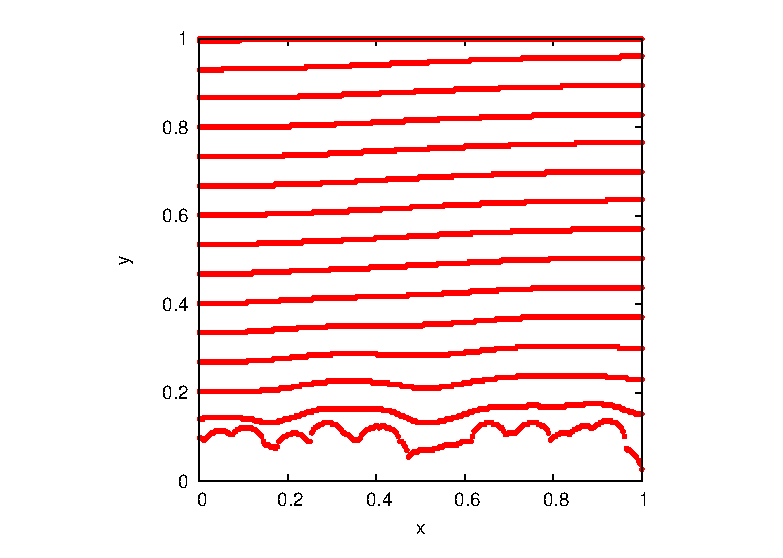
\includegraphics{trav_stability_wavefront.eps}
  \caption{The wavefront shape of multiple timesteps.
    Each wavefront has a difference in time by 2, i.e. they are at $t = 4, 6, 8, \ldots, 58, 60$. 
    The simulation results are the same as the previous Figures, using the default parameter values with a grid size $513 \times 513$.
    }
  \label{fig:trav_wavefront}
\end{figure}

Another interesting item to investigate is the actual shape of the wavefront.
Figure \ref{fig:trav_wavefront} shows only the wavefront shape for multiple timesteps.
The wavefront shape is the same dataset of points used to calculate the standard deviaiton of the wavefront interface.
Of interest is that the wavefront seems to move at a constant speed, since each wavefront shown is equidistance from the next.


%!% Maybe need to try other types of initial conditions to say this for sure...
%!% Or maybe just run this same experiment 5 or so times to get a better sample and then just show the stddev of all 5 on a single graph. If they all converge to 0ish then that looks pretty strong.


%%%%%%%%%%%%%%%%%%%%%%%%%%%%%%%%%%%%%%%%%%%%%%%%%%%%%%%%%%%
%!% Here I kinda want to show how the wavespeed dectector script works versus when I use the gnuplot fitting to calculate the wavespeed approximation.
%!% So here a mention the difference between each calculation and then show the horizontal translation graph for both the script and the fitted wavespeed.
%Show computations for the wave speed

%%%%%%%%%%%%%%%%%%%%%%%%%%%%%%%%%%%%%%%%%%%%%%%%%%%%%%%%%%%
\subsection{Parameter Effect on Wavespeed}

The travelling wave solutions seen before have all existed for a single set of parameters.
Here the four main system parameters, $\delta$, $\kappa$, $\nu$, and $\gamma$ are independent varied and the effect on the travelling wave solutions are observed.
From this we can also see how the wavespeed of the travelling wave solution changes as a function of the different model parameters.

%!% section 1.2.4:  each of these four parameters has a specific biological/physical meaning. You should explicitly state how the the wave speed qualitatively depends on increasing these biological parameters

\begin{figure}[h!tb]
  \centering
  \begin{tabular}{c c}
    \includegraphics[scale=0.55]{parameter_speed_delta.eps} &
    \includegraphics[scale=0.55]{parameter_speed_kappa.eps} \\
    (a) & (b) \\
    \includegraphics[scale=0.55]{parameter_speed_nu.eps} &
    \includegraphics[scale=0.55]{parameter_speed_gama.eps} \\
    (c) & (d) 
  \end{tabular}
  %!% Figure 1.14. the fonts i think are too small; these changes can be made later, not crucial for approving the thesis for defense
  \caption{The value of $c$ as parameter (a) $\delta$, (b) $\kappa$, (c) $\nu$, and (d) $\gamma$ are changed. 
    Note that (a) and (b) have logscales due to the selection of parameter values.
    Each of these were calculated with the same setup as the travelling solution previously done.
    The grid size for each was $513 \times 4$ and a time step of $\Delta t = 0.001$ was used.}
  \label{fig:parameter_speed}
\end{figure}

For this an automated script was created that checks, for each timestep, if $M$ is travelling wave solution based on the solution of $M$ from a number of timesteps previous.
From this check, a wavespeed needs to be approximated based on the distance between the two solutions.
If this approximated wavespeed is matched throughout all the x values, then a travelling wave solution is assumed to exist at that timestep.
With this script, we can try the same simulation as Figure \ref{fig:trav_wave_solution} with different parameter values.

For each parameter, $\delta$, $\kappa$, $\nu$, $\gamma$, the range of values choosen were arbitrarily.
Figure \ref{fig:parameter_speed} shows the results of the wavespeed for each parameter changes.
Mainly it was so that the solution did not progegate too fast and hit the end of the region before developing into a full travelling wave solution.
Generally when the travelling wave does not form it is because the wave front propegates to the end of the region faster then the tail of the travelling wave can decrease to 0.
In the case of $\nu$, any larger values then the selected range resulted in biomass that died faster then it could grow, and thus no travelling wave solution exists.
There did not appear to be any cases were a travelling wave solution could not form.

Since, for each of the choosen parameters, a travelling wave solution was seen to exist, it can be said that the choice of parameter in Figure \ref{fig:trav_wave_solution} was not the only reason for the travellin wave solutions existance.

%!%Explain that the wavespeed is characteristic of how fast the biomass is moving, so the parameters that directly affect the biomass-growth/dea/th etc. would change wavespeed the most.


